\documentclass[letterpaper]{article}
\usepackage{natbib,alifexi}
\usepackage[T1]{fontenc}
\usepackage{lmodern}
\usepackage[utf8]{inputenc}
\usepackage{abstract}
\usepackage{textcomp}
\usepackage{amsmath}
\usepackage{graphicx}
\usepackage{placeins}

\title{Étude d\textquotesingle algorithmes pour la détection de la tonalité de fichiers musicaux et implémentation en Clojure}
\author{Antoine Passemiers$$ \\
\mbox{}\\
$$Université Libre de Bruxelles \\
apassemi@ulb.ac.be}

\begin{document}
\maketitle

\renewcommand{\abstractname}{Résumé}    % Change the abstract title
\renewcommand\bibname{Bibliographie}        % Change the bib title
\renewcommand{\refname}{Bibliographie}



\begin{abstract}

Le projet consiste en la discussion de différents algorithmes relatifs à la détection 
automatisée de tonalité de fichiers musicaux, le prototypage de ceux-ci en Python,
ainsi qu\textquotesingle une réflexion sur l\textquotesingle adaptabilité de ces derniers avec le paradigme fonctionnel.
Le choix de l\textquotesingle algorithme a concevoir selon l\textquotesingle approche fonctionnelle sera basé
sur des critères de rapidité d\textquotesingle exécution et de précision de la détection. 
L\textquotesingle algorithme final sera alors implémenté en Clojure.

\end{abstract}

\section*{1. Introduction}

La tonalité d\textquotesingle une oeuvre musicale se caractérise par
l\textquotesingle ensemble des sons formant une même gamme diatonique. 
A la différence de la gamme, où les sons se succèdent de façon contigüe,
la tonalité (ou ton) regroupe des sons qui peuvent être disjoints et/ou superposés \citep{AD}.
En conséquence, nous nous intéressons à l\textquotesingle analyse de mélodies polyphoniques, 
où plusieurs notes peuvent être jouées en même temps.\\

En particulier, nous allons nous pencher sur deux catégories d\textquotesingle algorithmes :
ceux basés sur des modèles cognitifs, et ceux incluant des notions d\textquotesingle 
apprentissage automatique. Les premiers tentent d\textquotesingle intégrer au mieux les connaissances
de la théorie musicale et reposent sur la façon dont les personnes reconnaissent les différentes tonalités,
alors que les seconds utilisent l\textquotesingle inférence statistique pour déterminer celles-ci.\\

L\textquotesingle approche cognitive utilisée pour la détection de la tonalité repose en partie
sur la solution proposée par Ibrahim Sha\textquotesingle ath lors 
de la conception du logiciel KeyFinder \citep{IS}. La précision de la détection est évaluée 
à l\textquotesingle aide d\textquotesingle une base 
de données, constituée de 250 fichiers musicaux au format wav, dont les tonalités sont connues
et inscrites dans un fichier csv. Ces fichiers font partie de ceux utilisés par 
Ibrahim Sha\textquotesingle ath dans le cadre de sa recherche.\\

Pour ce qui est de la partie apprentissage automatique, les méthodes présentées seront principalement
en lien avec les modèles de Markov cachés. Leur évaluation se fera en divisant la base de données en
un jeu de données d\textquotesingle apprentissage et un jeu de données de validation (respectivement
60 \% et 40 \% du jeu de données d\textquotesingle origine). Ce mini-mémoire se voulant concis et 
centré sur les objectifs décrits, le lecteur est supposé déjà disposer de connaissances suffisantes en 
apprentissage automatique, en théorie musicale et en traitement logiciel de signaux.

TODO : \citep{SP} \citep{AT} -> Partie 2.1.1.

\section*{2. Considérations théoriques}

\subsection*{2.1. Pré-traitement}

Le signal audio est premièrement extrait du fichier wav, puis la moyenne entre les 
deux canaux est effectuée si le fichier a été enregistré en stéréo. En effet il n\textquotesingle
est pas nécessaire de prendre en compte le panoramique puisque celui-ci n\textquotesingle a que 
peu d\textquotesingle influence sur la mélodie dans le domaine spectral. 
Étant donné que les notes jouées sont uniquement caractérisées par leur fréquence fondamentale,
il n\textquotesingle est pas nécessaire de considérer l\textquotesingle entièreté du spectre
du fichier musical. De fait, la fréquence d\textquotesingle échantillonnage est abaissée à un dixième 
de la fréquence standard (4410 Hz), mais ce sous-échantillonnage est susceptible de provoquer des
phénomènes d\textquotesingle aliasing. La solution de Sh\textquotesingle ath implique de
gérer les problèmes d\textquotesingle aliasing sonore par l\textquotesingle application 
d\textquotesingle un filtre passe-bas. La taille de la fenêtre temporelle est un hyper-paramètre fixé durant
l\textquotesingle évaluation de l\textquotesingle algorithme. \citep{IS}

\subsection*{2.2. Estimation spectrale}

Il existe deux catégories de techniques d\textquotesingle estimation de densité spectrale : les méthodes paramétriques et les méthodes non-paramétriques.


\subsubsection*{2.2.1. Constant-Q Transform (CQT)}

Avant de procéder à l\textquotesingle estimation de la CQT, une fenêtre de Blackman est appliquée sur les données observées afin d\textquotesingle
 éviter les distortions spectrales dues à l\textquotesingle étroitesse de la fenêtre (et au principe d\textquotesingle incertitude d\textquotesingle Heisenberg).
Le spectre est alors approximé à l\textquotesingle aide de la transformée de Fourier rapide (FFT). L\textquotesingle intuition derrière la Constant-Q 
Transform (CQT)
est de penser que les coefficients de la FFT dont les fréquences ne correspondent pas à des notes de musique prennent plus de poids que les autres
coefficients. Ceci doit être réajusté en appliquant des fenêtres spectrales centrées sur les notes de musiques. Pour chaque fenêtre, les coefficients résultants de cette opération sont alors sommés pour ne former qu\textquotesingle un seul coefficient spectral. L\textquotesingle ensemble des coefficients globaux
constitue alors la CQT.


\subsubsection*{2.2.2. Décomposition harmonique de Pisarenko (PHD)}



\citep{MA}

\subsubsection*{2.2.3. Estimation spectrale par moindres carrés}

Il est possible d\textquotesingle estimer le spectre par régression, au travers d\textquotesingle algorithmes n\textquotesingle exigeant
pas de grandes quantités de calcul. Parmi les algorithmes les plus importants résident celui de Vaníček et celui de Lomb-Scargle. Leur particularité est
de pouvoir traiter des données qui ne sont pas reçues à intervalles réguliers (la majorité des observations se font la nuit). En outre, contrairement à la transformée de Fourier rapide qui possède une résolution aussi précise que la fenêtre d\textquotesingle observation est grande, ces algorithmes
calculent un périodogramme dont la taille est fixée par le nombre de fréquences qui nous intéressent. Au plus le nombre de fréquences analysées est
élevé, au plus le temps d\textquotesingle exécution sera conséquent.

\begin{align}
\hat{\theta}_{k} = (A_{k}^{T} A_{k})^{-1} A_{k}^{T} y
\end{align}

Selon la méthode de Vanícek, le signal est supposé être centré sur zéro et représenter une combinaison linéaire de sinusoïdes et d\textquotesingle un bruit blanc.
Les coefficients de cette combinaison linéaire sont réunis dans un vecteur $\theta_{k}$, de telle manière que le signal équivaut à $y \approx A\theta_{k}$.
La matrice A est telle que chaque ligne de celle-ci constitue une sinusoïde de fréquence d\textquotesingle intérêt. Les coefficients sont alors finalement
donnés par l\textquotesingle équation 1. \citep{PS}\\

Le défaut de la méthode est de ne pas considérer les phases des fréquences concernées. En effet chaque sinusoïde contenue dans la matrice A
est supposée posséder une phase nulle. La méthode de Lomb-Scargle permet de résoudre ce problème en pré-calculant les phases des sinusoïdes
utilisées et en tenant compte au mieux de celles-ci lors du calcul du spectre. Le déphasage $\tau$ correspondant à la fréquence $f$ est donné par
l\textquotesingle équation 2. \citep{LS}

\begin{align}
\tan 2\pi f \tau = \frac{\sum\limits_{j=1} \sin 2\pi f t_{j}}{\sum\limits_{j=1} \cos 2\pi f t_{j}}
\end{align}

Tout comme dans la méthode de Vanícek, la régression consiste en la recherche de coefficients qui expliquent au mieux le signal sous la forme d\textquotesingle
une pondération de sinusoïdes. Le coefficient associé à la fréquence $f$ est donné par l\textquotesingle équation 3 :

\begin{align}
\Delta R(f) = \frac{(YC)^{2}}{CC} 
+ \frac{(YS)^{2}}{SS}
\end{align}

Les valeurs CC et SS peuvent être pré-calculées, car les fréquences d\textquotesingle intérêt ne changent pas d\textquotesingle un fichier
à l\textquotesingle autre.

\begin{align}
CC = \sum\limits_{j=1} \cos^{2} 2\pi f (t_{j} - \tau)
\end{align}

\begin{align}
SS = \sum\limits_{j=1} \sin^{2} 2\pi f (t_{j} - \tau)
\end{align}

Les valeurs YC et YS cherchent à mesurer respectivement les niveau d\textquotesingle orthogonalité du signal $y$ avec une sinusoïde déphasée de $\pi / 2$
et avec une sinusoïde de phase nulle. Ces sinusoïdes peuvent également être pré-calculées. Les formules permettant de calculer YC et YS sont :

\begin{align}
YC = \sum\limits_{j=1} y_{j}\cos 2\pi f (t_{j} - \tau)
\end{align}

\begin{align}
YS = \sum\limits_{j=1} y_{j}\sin 2\pi f (t_{j} - \tau)
\end{align}

Ainsi, les seules opérations restantes lors de l\textquotesingle exécution de l\textquotesingle algorithme sont les produits scalaires entre les
sinusoïdes et le signal délimité par la fenêtre glissante, ce qui réduit drastiquement la quantité de calculs requis pour l\textquotesingle estimation du spectre.

\subsubsection*{2.2.4. Autres méthodes}

TODO : Cepstre, spectre de puissance, ...

\subsection*{2.3. Prédiction de la tonalité}

Une fois le spectre estimé, celui-ci est compacté dans un vecteur chromatique composé de douze coefficients. Dans le cadre de l\textquotesingle évaluation de l\textquotesingle algorithme, il a été trouvé que 6 octaves suffisent à approximer le spectre : l\textquotesingle ajout d\textquotesingle une septième octave n\textquotesingle améliore pas la précision des prédictions. De fait, le spectre dont la résolution est de 72 coefficients (12 x 6 octaves) est redimensionné en une matrice $M_{i, j}$ de dimensions (6 x 12). Enfin, le vecteur chromatique $C_{i}$ est obtenu en formalisant la méthode élaborée par Sha\textquotesingle ath :

\begin{align}
C_{i} = (1 - p) * \max_{j} M_{i, j} + p * \sum_{j} M_{i, j}
\end{align}

où p est un hyper-paramètre déterminé durant l\textquotesingle évaluation/validation de l\textquotesingle algorithme. La dernière étape consiste alors à identifier localement la tonalité sur base unique de ce vecteur chromatique. Différentes méthodes ont été discutées, la première se base sur la méthode de
Sh\textquotesingle ath alors que les suivantes reposent sur des algorithmes d\textquotesingle apprentissage automatique.

\subsubsection*{2.3.1. Modèle cognitif}

Cette solution repose sur les expériences menées par Carol L. Krumhansl et Lola L. Cuddy sur la perception des tonalités chez l\textquotesingle Homme.
Des gammes incomplètes ont été jouées, suivies de notes additionnelles que les sujets devaient évaluer sur leur capacité à compéter ces gammes. 
Les scores ont été moyennés pour donner les deux graphiques suivants :

\FloatBarrier

\begin{figure}[h!]
\begin{center}
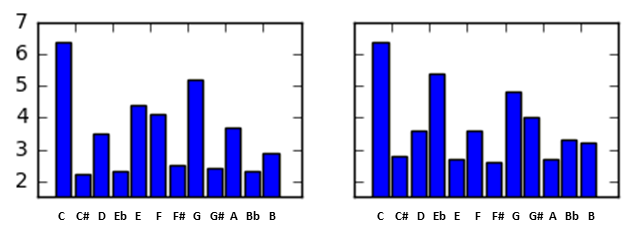
\includegraphics[width=3.1in,angle=0]{imgs/Krumhansl.png}
\caption{Profils de tonalités dérivés de l\textquotesingle expérience de Krumhansl, et représentant respectivement la gamme do majeur
et la gamme do mineur.}
\label{fig1}
\end{center}
\end{figure}

Bien que ces deux profils de tonalités fournissent des résultats satisfaisants lorsque le spectre est estimé à l\textquotesingle aide de la CQT, il ne sont pas adaptés lorsque la méthode de Lomb-Scargle est utilisée, car il a été observé que les coefficients renvoyés par cette dernières sont globalement plus equidistribués. Cette distribution doit se refléter dans les profils de tonalité, c\textquotesingle est pourquoi l\textquotesingle algorithme a été évalué plusieurs fois jusqu\textquotesingle à obtenir les profils fournissant les meilleurs résultats, et donnés ci-dessous :

\begin{figure}[h!]
\begin{center}
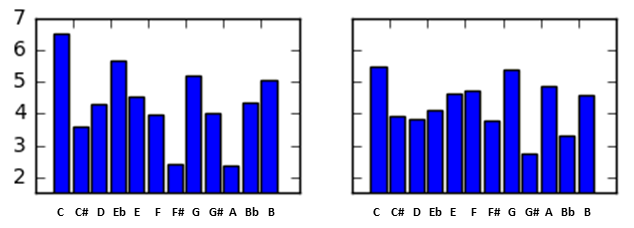
\includegraphics[width=3.1in,angle=0]{imgs/Custom.png}
\caption{Meilleurs profils de tonalités, déterminés empiriquement}
\label{fig1}
\end{center}
\end{figure}

\FloatBarrier

\subsubsection*{2.3.2. Modèles de Markov Cachés (HMM)}

Les modèles de Markov cachés sont des machines à états discrets cherchant à représenter des séries multivariées par
leurs distributions, ainsi que par les probabilités de transition entre les états cachés de la machine. De plus, chaque état
caché de cette dernière possède ses propres probabilités d\textquotesingle émission. Contrairement à des modèles d\textquotesingle
apprentissage automatique plus populaires tels que les réseaux de neurones ou les machines à vecteurs de support,
les HMM sont capables de traiter des séquences de longueur non fixée. Cette caractéristique est appréciable dans le cadre
de l\textquotesingle analyse de morceaux de musique, qui ont des durées de nature très variables.

TODO : \citep{JP} \citep{DR}

\subsubsection*{2.2.3. Modèles de Markov Cachés de type entrée-sortie (IO-HMM)}

TODO : \citep{YB}

\subsection*{2.4. Évaluation}

Dans le cadre de ce travail, seules les douze gammes majeures et leurs douze gammes mineures relatives correspondantes sont considérées.
Deux mesures différentes sont utilisées afin d\textquotesingle évaluer la précision de l\textquotesingle algorithme : 
la précision (le ratio du nombre de prédictions correctes sur le nombre de fichiers analysés), ainsi que l\textquotesingle indice du MIREX.
Ce dernier est égal à une combinaison du nombre de bonnes prédictions (avec une pondération de 1,0), du nombre de prédictions décalées de
5 demi-tons (pondération de 0,5), du nombre de prédictions décalées de 4 demi-tons (pondération de 0,5), du nombre de prédictions de gamme
relative (pondération de 0,3), et du nombre de prédictions de gamme parallèle (pondération de 0,2).


\subsubsection*{2.5. Résultats}

\FloatBarrier

\begin{table}[h!]
\center{
\begin{tabular}{|c|c|c|}\hline
Méthode & Précision & MIREX \\ \hline\hline
CQT + profiles & 30,7\%  & - \\
Lomb-Scargle + profiles & - & - \\
CQT + HMM & -- & -- \\
FFT + IO-HMM & -- & -- \\
CQT + IO-HMM & -- & -- \\ 
Lomb-Scargle + IO-HMM & -- & -- \\ 
\hline
\end{tabular}
}
\vskip 0.25cm
\caption{Évaluation des méthodes présentées selon la précision et l\textquotesingle indice du MIREX}
\end{table}

\FloatBarrier

\section{3. Implémentation en Clojure}

TODO : \citep{SK}


\footnotesize
\bibliographystyle{apalike}
\bibliography{thesis}


\end{document}